\section{Probase}
Probase is a probabilistic knowledge base, built by 
extracting pairs of \textit{isA} relationship of concepts 
from web pages. In Probase, concepts are stored in a 
taxonomic manner. Currently, it contains around 2.7 
million concepts that were extracted from more than 1 
billion web pages. A concept in Probase can be seen as 
a representation of object in real world. An instance 
can also be considered as a single concept, which cannot 
be instantiated into other concepts or instances. Figure 
\ref{fig:exampleProbase} shows the example for this relation.

\begin{figure}[h]
\centering
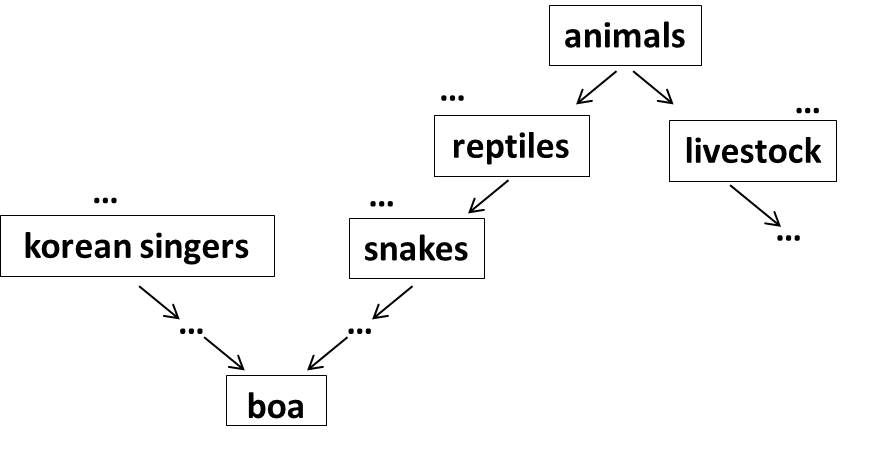
\includegraphics[scale=0.3]{images/Figure2}
\caption{Example of concepts and instances in Probase}
\label{fig:exampleProbase}
\end{figure}

We can see from this figure, that ``animals'', ``livestocks'', 
``reptiles'', ``snakes'', ``korean singers'' are regarded as 
concepts, and ``boa'' as an instance. A concept may be a 
subconcept of other concept, e.g. ``snakes'' is a subconcept 
of ``animals''.

The distinctive aspect of Probase compared with other knowledge 
bases is that, in Probase, the relation between a concept and 
subconcept or a concept and an instance is not defined in a strict 
well-defined manner. Each relation is given a probability value 
which measure the \textit{value} of the relationship. The first 
value called \textit{plausibility} value, measures how strong or 
certain we are that a concept and a subconcept is actually related. 
Take an example of pair (``animals'',``reptiles''). The plausibility 
value tells us how strong that the 'reptiles' is seen as 'animals' or 
how certain we are that 'reptiles' is indeed 'animals'. This degree 
of uncertainty is important since it represents how exactly the 
concepts in the real world is attached to each other.

Another value that is a subject of interest to us in this work is 
the \textit{typicality} value. It measures how strong the relation 
between a concept and an instance. We take use of this value as one 
of the components to measure the relevancy between the concepts in 
user query and the instances found in queries from query log. The 
value is derived as:
\[Typicality\textnormal{-}value(i, c) = \frac{n(i, c)}{n(c)+\alpha}\]
where $i$ is an instance and $c$ is a concept. The $n(i,c)$ is the 
frequency of the occurrence of instance $i$ and concept $c$ together 
in extracted pairs from web pages, and $n(c)$ is the frequency of the 
occurrence of concept $c$ in all pairs. The value $\alpha$ is used 
to smooth the score and to avoid the high typicality value of a 
concept $c$ that only have one instance $i$, which can be harmful 
if the relationship is supposed to be small. To show how typicality 
value can be used, take an example of an instance ``boa''. The 
typicality value of pair (``boa'',``snakes'') is 0.0138 while the pair 
(``boa'',``korean singers'') has typicality value of 0.00197. From 
this result, we can see that ``boa'' is more likely known as a name 
of a snake than as the name of a singer.
\\
\\


%439871 boa
%1720113 snakes
%973216 korean singers
%
%439871	61
%1720113	0.0138181818181818
%993835	0.00486144871171609
%973216	0.0019723865877712

